%!TEX root = ../../main.tex
%----------------------------------------------------------------------------
\chapter*{Project Description}\label{chap:project_description}
%----------------------------------------------------------------------------

\addcontentsline{toc}{chapter}{\nameref{chap:project_description}}

The goal of the project is the development of a robot production facility that packs LEGO orders for a company. The LEGO orders describe a number of particular bricks in different colors and shapes, which are to be selected and packed for delivery. 

The system consists of the following elements, performing the tasks listed below:
\begin{itemize}
	\item Manufacturing Execution System (MES): The central server managing order processing and scheduling. 
	\item Robot cells: Sorting and packing the LEGO bricks. 
	\item Mobile robots: Transporting unsorted as well as sorted and packed LEGO bricks. 
	\item LEGO brick dispenser: Supplying the LEGO bricks. 
	\item Marker locator: Positioning system for tracking the mobile robots. 
	\item Safety system (Pilz Safety Eye): Accident prevention.
\end{itemize}

The connection of these system elements is shown in figure \ref{fig:overall_system_diagram}.
    \begin{figure}[H]
        \centering
        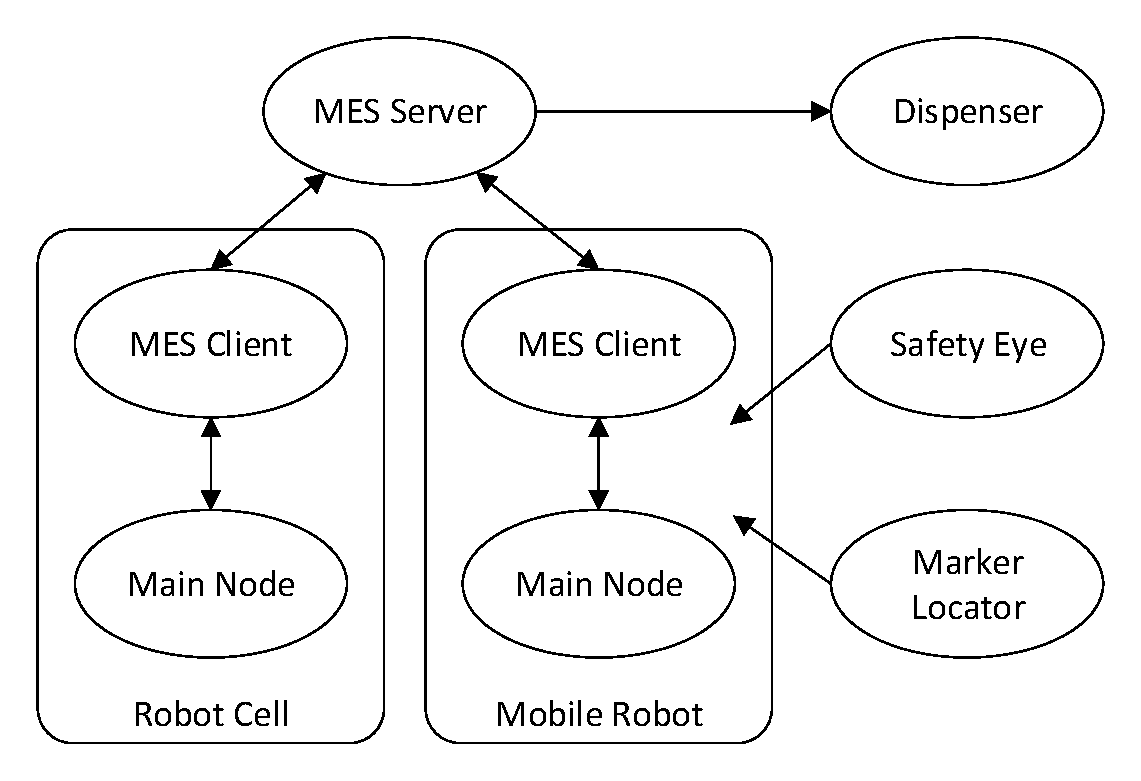
\includegraphics[width=0.7\textwidth]{overall_system.pdf}
        \caption{Overall connection of the system elements}
        \label{fig:overall_system_diagram}
    \end{figure}

%%% Local Variables:
%%% mode: latex
%%% TeX-master: "main"
%%% End:
